\documentclass{article}
\usepackage{soulutf8}
%\renewcommand{\st}[1]{}
%\usepackage[scale=.75]{geometry}
\usepackage{placeins}
\usepackage{amsthm,amssymb,hyperref,marginnote}
\usepackage{subfig}
\usepackage{enotez}
\setenotez{counter-format=Alph}
\usepackage{luatodonotes}%\usepackage{todonotes}%
\usepackage{xcolor}
\newcommand{\nb}[1]{\todo[color=blue!60!black,shadow]{#1}}

\theoremstyle{definition}
\newtheorem{definition}{Definition}
\usepackage{amsmath}
\title{Heterogeneous mempool \DAG[s]}
\author{Typhon Team Heliax}
\date{\today}
\usepackage{lmodern}
\usepackage[utf8]{inputenc}
\usepackage[T1]{fontenc}
\usepackage{xspace}
% macros
\newcommand{\tnote}[1]{
  \marginnote{\footnotesize #1}%
}
\newcommand{\rtnote}[1]{%
  \reversemarginpar%
  \tnote{#1}%
  \normalmarginpar%
}
  
\newcommand{\DAG}[1][]{\textsc{dag}#1\xspace}
\newcommand{\aka}[1][]{a.k.a.\xspace}
\newcommand{\ie}[1][]{\emph{i.e.}, }
\newcommand{\eg}[1][]{\emph{e.g.}, }
\newcommand{\fig}[1][]{Fig.~}
\newcommand{\Learner}{%
  % the set of learners
  \ensuremath{L}
}
\newcommand{\Q}[1]{%
  % trust live
  Q_{#1}%
}
\newcommand{\rough}[1][]{%
  %\fbox{\color{blue!70!black}!!}%
  {\color{blue!70!black}\ul{#1}}
}
\newcommand{\circledX}[1]{\tikz[baseline={(x.south)}]{\node[circle,draw,inner sep=.5pt,outer sep=0pt](x){\tiny #1};}}
\usepackage{newunicodechar}
%\newunicodechar{}{\ensuremath{}}  
\newunicodechar{₁}{\ensuremath{{}_1}}
\newunicodechar{₂}{\ensuremath{{}_2}}
\newunicodechar{₃}{\ensuremath{{}_3}}
\newunicodechar{₄}{\ensuremath{{}_4}}
\newunicodechar{₅}{\ensuremath{{}_5}}
\newunicodechar{★}{\ensuremath{*}~}
\newunicodechar{ }{~}
\newunicodechar{①}{\circledX 1}
\newunicodechar{“}{``}
\newunicodechar{”}{''}
\newunicodechar{②}{\circledX 2}
\newunicodechar{ₐ}{\ensuremath{{}_a}}
\newunicodechar{ₚ}{\ensuremath{{}_p}}
\newunicodechar{‼}{\rough}
\newunicodechar{‽}{\ensuremath{?!}}
\newunicodechar{↑}{\ensuremath{\uparrow}}  
\newunicodechar{⇑}{\ensuremath{\Uparrow}}  
\newunicodechar{♯}{\ensuremath{\sharp%\hat\#
}}  
\newunicodechar{∅}{\ensuremath{\varnothing}}
\newunicodechar{≠}{\ensuremath{\neq}}              
\newunicodechar{∩}{\ensuremath{\cap}}              
\newunicodechar{≡}{\ensuremath{\equiv}}              
\newunicodechar{∈}{\ensuremath{\in}}
\newunicodechar{ℝ}{\ensuremath{\mathbb{R}}}
\newunicodechar{↔}{\ensuremath{\leftrightarrows}}    
\newunicodechar{→}{\ensuremath{\rightarrow}}
\newunicodechar{←}{\ensuremath{\leftarrow}}
\newunicodechar{⇒}{\ensuremath{\Rightarrow}}
\newunicodechar{∀}{\ensuremath{\forall}}
\newunicodechar{‌}{\allowbreak }
\newunicodechar{‍}{{}}                                

\usepackage{tikzpeople}%‼ for evil validators etc. 

\usepackage{tikz}
\usetikzlibrary{shapes,positioning,fit,backgrounds}
\usetikzlibrary{patterns,intersections,calc}
\newcommand{\qs}[1][~]{\tikz[baseline={([yshift=0pt]theNode.base)}]{\node[rectangle,
,double,inner sep=.5pt,outer sep=0pt,fill=black] (theNode){\textcolor{white}{\footnotesize \bf q#1}};}
}
\newcommand{\bk}[1][green!60!black]{\tikz[baseline={([yshift=0pt]theNode.base)}]{\node[regular polygon, regular polygon sides=6
,double,inner sep=.5pt,outer sep=0pt,fill=#1] (theNode){\textcolor{white}{\footnotesize \bf bk}};}}
\newcommand{\ac}{\tikz[baseline={([yshift=0pt]theNode.base)}]{\node[regular polygon, regular polygon sides=6
,double,inner sep=.5pt,outer sep=0pt,fill=black] (theNode){\textcolor{white}{\footnotesize \bf a}};}}

\newcommand{\hd}[1][ ]{%
  \ifthenelse{\equal{#1}{}}%
  {\tikz[baseline={([yshift=0pt]theNode.base)}]{
      \node[rectangle,inner sep=1.5pt,outer sep=0pt,double] (theNode){\textcolor{black}{\footnotesize \bf \ul{HD}}};
    }}%
  {\tikz[baseline={([yshift=0pt]theNode.base)}]{
      \node[rectangle,double,inner sep=1.5pt,outer sep=0pt,double,draw] (theNode){\textcolor{black}{\footnotesize \bf HD}};
      
    }}%
}
\newcommand{\wh}[1][ ]{%
  \tikz[baseline={([yshift=0pt]theNode.base)}]{%
    \ifthenelse{\equal{#1}{ }}%
    {\node[rectangle,fill=black,inner sep=1.5pt,outer sep=0pt] (theNode){\textcolor{white}{\footnotesize \bf WH}};}%
    {\node[rectangle,draw,fill=lightgray,inner sep=1.5pt,outer sep=0pt] (theNode){\textcolor{black}{\footnotesize  WH}};}%
  }%
}
\newcommand{\tx}[1][]{\tikz[baseline={([yshift=0pt]theNode.base)}]{\node[ellipse,fill=black,inner sep=.5pt,outer sep=0pt] (theNode){\textcolor{white}{\footnotesize \bf TX}};}#1}
\newcommand{\es}{\tikz[baseline={([yshift=0pt]theNode.base)}]{\node[ellipse,fill=white,draw,thick,inner sep=.5pt,outer sep=0pt] (theNode){\textcolor{black}{\footnotesize TX}};}}
\newcommand{\rnd}{\ensuremath{\mathrm{rnd}}}
\newcommand{\cnt}{\ensuremath{\mathrm{cnt}}}
% \usepackage{ebgaramond}
% \usepackage[cmintegrals,cmbraces]{newtxmath}
% \usepackage{ebgaramond-maths}
% \usepackage{amssymb}
% \usepackage{fontspec}
% \setmainfont{Asana-Math}

%https://tex.stackexchange.com/questions/425098/which-opentype-math-fonts-are-available
\usepackage{comment}
%\includecomment{comment}
\begin{document}
\renewcommand{\todo}[2][]{}
\begin{comment}
\maketitle

\tableofcontents
\section{Introduction}

\paragraph{Motivation%
\endnote{%
  Paragraph 1: Motivation.
  At a high level, 
  what is the problem area you are working in and why is it important? 
  It is important to set the larger context here. 
  Why is the problem of interest and importance to 
  the larger community?
}%
}
Bridges%
\st{ suck} %
have been the source of sorrow in the past. 
Even if they do work as intended, 
at best, they connect a single pair of chains. 
Building bridges between every pair of chains
is ‼[expensive]. %
We want to enable
any number of participants with assets on several
different ledgers\endnote{%
- base chains
- root chains
- ledgers 
} to ‼[“interact” “directly”].
\todo{explain “interact” “directly”}
%\newcommand{\dl}[1][]{\textsc{dl}#1\xspace}(\dl[s])
\todo[inline]{
  argumentation flaw:
  if we have a base ledger count of~\(n\), 
  we will have a quadratic number of chimera chains as well,
  i.e., (at least) one learner for each chimera chain. 
}
\paragraph{Probblem statement%
  \endnote{%
    Paragraph 2:
    What is the specific problem considered in this paper? 
    This paragraph narrows down the topic area of the paper. 
    In the first paragraph you have established general context and importance.
    Here you establish specific context and background. 
  }%
}
‼[
\tt How to enable any number of actors to interact directly
with moderate ressource consumption and suitable latency, 
us-ing only a “minimal” number validators on the involved base ledgers.
%
]
The ideal solution would be 
the atomic execution of a single transaction that
makes reference to all invovled base ledgers.%
\footnote{%
  This assumes counterparty discovery 
  before the transaction  is crafted.
}%
\xspace
Can we operate a protocol
that strikes a good compromise between
the number of validators necessary to order (and execute) transactions,
not spending more ressources than complete pair-wise bridging?




\subsection{Overview}
Roughly, we have two complementary protocols running concurrently: 

\begin{figure}[htb]
  \centering
  
  \begin{tikzpicture}
    \node[draw] (avl) {transaction data};

    \node[draw,right=1ex of avl] (dag) {``causal'' \DAG structure};
    \begin{pgfonlayer}{background}
    \node (x) [fill=lightgray,fit=(avl)(dag)] {};
  \end{pgfonlayer}
  \node[above=2ex of x,draw,double] {uniqueness of headers};
\end{tikzpicture}\protect\todo{where to put the signed quorums ?!}
  \caption%
  [Interdependence of availability and integrity]%
  {Illustration of the interdependence of the availability and integrity protocols}
  \label{fig:availability-n-integrity}
\end{figure}
 \begin{enumerate}
 \item the availability protocol; and
 \item the integrity protocol. 
 \end{enumerate}
 The availability protocol makes sure
 that transaction data is made available as long as necessary.
 The integrity protocol makes sure that 
 each validator can only produce one block in each of its (local) rounds. 
 However, % 
 the integrity protocol produces additional data, %
 besides transactions, 
 which leads to additional data to be taken care of by the availability protocol.


\section{Architecture and communication patterns}
\label{sec:communication-patterns}
 We incorporate Narwhal's~\cite{NT} 
 scale out architecture%in our availability protocol 
 : %
 each validator has a unique \emph{primary} and % 
 a number of \emph{workers} % 
 (see \fig\ref{fig:validators})%
 . 
\begin{figure}[htb]
  \centering

validator:\(\left\{\begin{tikzpicture}[baseline={(p.south)},remember picture]
    \node[circle,draw,inner sep=1.5ex] (p) at (5.5,1.2) {p};
    \foreach \i in {1,...,10}{
      \coordinate (p_\i) at  (p.160+20*\i);
    }
    \foreach \i in {1,...,10}{
      \node[rectangle,fill=lightgray](w_\i) at (\i,0){\(w_{\i}\)};
      \draw[->] (w_\i.north) .. controls +(0,.2) .. (p_\i);
    }
    \begin{pgfonlayer}{background}
      \node[rounded corners,fill=blue!30!white,inner sep=2ex] (background) [fit=(w_1.south west)(w_10.south east)(p)] {};
    \end{pgfonlayer}
  \end{tikzpicture}\right.\)

\vspace{4ex}

\tikz[remember picture]{\node[rectangle,fill=gray,draw] (c) {client};}\hfill~\\

\vspace{4ex}

validator:\(\left\{\begin{tikzpicture}[baseline={(q.north)},remember picture,yscale=-1]
    \node[circle,draw,inner sep=1.5ex] (q) at (5.5,1.2) {q};
    \foreach \i in {1,...,10}{
      \coordinate (q_\i) at  (q.200-20*\i);
    }
    \foreach \i in {1,...,10}{
      \node[rectangle,fill=lightgray](v_\i) at (\i,0){\(v_{\i}\)};
      \draw[->] (v_\i.south) .. controls +(0,.2) .. (q_\i);
    }
    \begin{pgfonlayer}{background}
      \node[rounded corners,fill=blue!30!white,inner sep=2ex] (background) [fit=(v_1.north west)(v_10.north east)(q)] {};
    \end{pgfonlayer}
    % --------------------------------------------------------------------------------
    \begin{scope}[overlay,thick]
          \foreach \j in {1,...,10}
    \draw[<->] (v_\j) -- (w_\j);

    \draw[<->] (c.-15) .. controls +(2,0) and +(-1,-1) .. (v_3.north west);
    \draw[<->] (c.15) .. controls +(2,0) and +(-1,1).. (w_7.south west);
    \draw[<->] (p) -- (q);
    \end{scope}
  \end{tikzpicture}\right.\)
  \caption{The structure and communication patterns of validators}
  \label{fig:validators}
\end{figure}



\section{Preliminaries}
\label{sec:preliminaries}
\todo[inline]{%
  ``copy'' relevant parts of % 
  the heterogeneous paxos tech report%
}

Let us fix an arbitrary learner graph. 

\begin{definition}[Global Weak Quorum]
  \label{def:global-weak-quorum}
  A %
  \emph{global weak quorum} %
  is a set~\(X\) that is a weak quorum for each learner,  %
  i.e., \(X ∩ qₐ ≠ ∅\) %
  for every learner~\(a ∈ \Learner\), and %
  all \(qₐ ∈ \Q{a}\).
\end{definition}

\begin{definition}[Universal Quorum]
  \label{def:universal-quorum}
  A universal quorum is a set
  that contains a qourum for each learner,
  \ie a set \(q\) such that \(q ∈ \Q a\)
  for all \(a ∈\Learner\). 
\end{definition}



\section{Worker actions}
\label{sec:worker-actions}
Every validator has the same number of workers. 
Thus,
each worker can be assigned a unique \emph{mirror worker} 
on every other validator.
We shall adopt the convention that
mirror workers of each other share the same subscript,
\eg in \fig\ref{fig:validators},
workers~\(w_2\) and~\(v_2\) are mirror workers of each other.
Workers are only tasked with “bookkeeping” matters: 
they keep track of (batches of) transactions,
their hashes,
and erasure coding shares;
they only pass on hashed data and header information 
to their primaries. 
Primaries never send messages back to their workers. 


\subsection{The pure availability protocol: worker actions}
\label{sec:base-protocol}
\todo[inline]{get rid of the broadcast of the availability certificates}
\todo[inline]{%
  maybe we need to ``announce'' headers, % 
  to avoid ``crossing'' of round numbers of learner%
}
\todo[inline]{%
  so, signed qourums are an ``output'' of the integrity protocol,
  and need to be made available (such that it is possible to create new headers). 
}

\todo[inline]{%
  worker hashes also should include an availability certificate %
  of the header creator's previous header %
}

\begin{description}
\item[Transaction collection (\tx{}←)] 
  \tnote{worker\\ ← client}
  Each worker keeps listening 
  for new transaction requests from clients.\footnote{%
    The bandwith and amount of storage for storing incoming transactions
    \emph{should} be big enough 
    to process all incoming transactions. 
    We share this assumption with Byzantine set consensus \cite{RedBelly}. 
    Transaction fees are one way to avoid flooding attacks,
    making the latter prohibitively expensive. 
  }
  Transactions should be buffered using reasonably fast memory. 
  \todo[inline]{When is the buffer %
  ①\emph{flushed} and/or %
  ②\emph{emptied} %
  ?
  Emptying not a concern in this paper / future work. 
  }

\item[Transaction distribution (\tx⇒)]
  \tnote{worker\\ ⇒ worker}
  Each worker “broadcasts” erasure coding shares of 
  every received transaction to mirror workers.
  In the simplest case\xspace% 
  ---the one we cover first---%
  this amounts to broadcasting the transaction.\footnote{ 
  However, 
  if we perform proper erasure coding,  
  it is not broadcasting in the strict sense:
  each mirror worker receives a different message. 
  We first cover the case of trivial erasure coding
  ‼[covering the case of proper erasure codining in ‽].
  }
  In general,
  transaction distribution can be divided into two steps.
  \todo[inline]{
    we might require a 
    \emph{position number} for
    transactions of the current batch, 
    and a sequence number (of the block to be produced)
  }
  \begin{description}
  \item[Erasure coding via copying (\es)]
    \tnote{[worker]}
    We first cover the case of trivial erasure coding, 
    in line with the description of the homogeneous case~\cite{NT}. %
    Thus, erasure coding shares of a transactions are simply copies. 
    We visually distinguish between “copies” of transactions
    from the “original” transaction supplied by the client,  
    using the symbols \tx\ and \es, respectively. 
%%%%%%%%%%%%%%%%%%%%%%%%%%%%%%%%%%%%%%%%%%%%%%%%%%%%%%%%%%%%%%%%%%%%%%%%%%%%%%%%%%%%%%%%%
    \todo[inline]{put fwd ref / future work }
%%%%%%%%%%%%%%%%%%%%%%%%%%%%%%%%%%%%%%%%%%%%%%%%%%%%%%%%%%%%%%%%%%%%%%%%%%%%%%%%%%%%%%%%%    
  \item[Copy distribution (\es⇒)] 
    \tnote{worker\\ ⇒ worker }
    Each share of the erasure code,
    \ie a copy of the transaction, 
    is sent to every mirror worker.%
    \endnote{
      elaborate on the distribution scheme,
      and how the destination of each earasure share is determined
      (for the general erasure coding).
    }%
    \xspace
    We tag each transaction with a \emph{sequence number},
    consisting of the validator round and 
    the position in the list of transactions for 
    the next block (header) in which the transaction will be included. 
    % so that it becomes clear in which order the 
    % transactions of the next block (header) will be listed. 
  \end{description}
  Note that copies of transactions are \emph{not} signed by the worker. 
  Signatures are deferred to until after the last transaction  
  of a validator round, 
  when the worker will sign the hash of the list of all broadcast transactions,
  called a \emph{worker hash}. 
  
\item[Worker hash compilation (\wh)]
  \tnote{(worker)}
  Towards the end of a “validator round”,\endnote{%
    Is there any such thing as “validator round”?\\
    - sequence number\\
    - validator height\\
    - ... 
  }%
  \xspace
  each worker produces its worker hash for the broadcast batch of transactions. 
  In detail,
  a worker hash consists of 
  \begin{itemize}
  \item the hash of the broadcast list of transactions,
  \item the number of transactions, and
  \item the round number,  
  \end{itemize}
  signed by the worker. 
  \endnote{\color{red}
    For general erasure coding:
    \em Does this need to includes for each receiving worker,
    the (hashes of the) erasure coding shares that 
    they should have available. ?
  }
\item[Worker hash broadcast (\wh⇒)] 
  \tnote{worker\\ ⇒ worker }  
  A worker broadcasts its most recent worker hash
  to mirror workers.
\item[Worker hash provision (\wh↑)]
  \tnote{worker\\ → primary}
  The most recent worker hash is sent to the primary 
  for inclusion into the next header. 
  \todo{
    How much “additional” information do we have 
    to include into the header
    such that signing a header certificate becomes meaningful?
  }
  
\item[Worker hash reception and checking ({\wh[]←})] 
  \tnote{worker\\ ← worker}  
  At any time, 
  a worker can receive a worker hash 
  from a mirror worker. 
  As a first reaction, 
  it checks whether enough 
  transactions have been received by the worker and, 
  if so, 
  whether the hash of the list of transaction matches the worker hash. 

\item[Worker hash forward ({\wh[]⇑})]
  \tnote{worker\\ → primary}  
  If a worker has successfully checked 
  the availability of the transactions of a received worker hash, %
  it “forwards” the worker hash to its primary.\footnote{%
    Validators will use this information 
    to send availability commitments to block headers of other primaries.
  }
\end{description}



\begin{figure}[htb]
  \centering
  \tikzstyle{every node}+=[outer sep=0pt,inner sep=1pt]
  \newcommand{\primaryDistance}{15ex}
  \newcommand{\workerPrimaryDistance}{1ex}
  \newcommand{\workerDistance}{3ex}
  \scalebox{.9}{%
  \footnotesize%
  \begin{tikzpicture}[scale=1.2]
    %%%%%%%%%%%%%%%%%%%%%%%%%%%%%%%%%%%%%%%%%%%%%%%%%%%%%%%%%%%%%%%%%%%%%%%%%%%%%%%% 
    % The message passing diagram of the availability protocol at genesis
    %%%%%%%%%%%%%%%%%%%%%%%%%%%%%%%%%%%%%%%%%%%%%%%%%%%%%%%%%%%%%%%%%%%%%%%%%%%%%%%%
    % first the time lines for primaries and their workers
    \coordinate (primaryAnchor) at (0,0);
    \foreach \p in {1,...,5} {
      \node[below=\primaryDistance of primaryAnchor,anchor=east] (p\p) 
      at (primaryAnchor) {\ensuremath{\text{primary}_\p}};
      \draw[->] (p\p) -- ++(10.4,0);
      \coordinate (workerAnchor) at ([yshift=-\workerPrimaryDistance]p\p.east);
      \foreach \j in {1,...,2} {
        \node[below=\workerDistance of primaryAnchor,anchor=east] (w\p_\j) 
        at (workerAnchor) {\ensuremath{\text{worker}_{\p,\j}}};
        \draw[->] (w\p_\j) -- ++(10.4,0) ;
        \coordinate (workerAnchor) at (w\p_\j.east);
      }
      \coordinate (primaryAnchor) at (p\p.east);
    }
    %%%%%%%%%%%%%%%%%%%%%%%%%%%%%%%%%%%%%%%%%%%%%%%%%%%%%%%%%%%%%%%%%%%%%%%%%%%%%%%% 
    % a first transaction tx1
    \node (tx1) at ([xshift=3.5ex]w1_1.east) {\tx₁};
    \draw[->,double,dotted,shorten >=-2ex] (tx1.200) ++ (200:1em) -- (tx1);
    \foreach \p in {2,...,5} {
      \node (es\p_1) at ([xshift=6ex-\p ex]tx1|-w\p_1) {\es₁};
      \draw[->] (tx1) -- (es\p_1) ;
    }
    % a bunch of transactions tx2-5 that will make it into WHs actually
    \node (tx2) at ([xshift=3*3.5ex]w3_2.east) {\tx₂};
    \draw[->,double,dotted,shorten >=-2ex] (tx2.200) ++ (200:1em) -- (tx2);
    \foreach \p in {1,2,4,5} {
      \node (es\p_2) at ([xshift=6ex-\p ex]tx2|-w\p_2) {\es₂};
      \draw[->] (tx2) -- (es\p_2) ;
    }
    \node (tx3) at ([xshift=5*3.5ex]w3_2.east) {\tx₃};
    \draw[->,double,dotted,shorten >=-2ex] (tx3.200) ++ (200:1em) -- (tx3);
    \foreach \p in {1,2,4,5} {
      \node (es\p_3) at ([xshift=6ex-\p ex]tx3|-w\p_2) {\es₃};
      \draw[->] (tx3) -- (es\p_3) ;
    }
    \node (tx4) at ([xshift=7*3.5ex]w3_1.east) {\tx₄};
    \draw[->,double,dotted,shorten >=-2ex] (tx4.200) ++ (200:1em) -- (tx4);
    \foreach \p in {1,2,4,5} {
      \node (es\p_4) at ([xshift=6ex-\p ex]tx4|-w\p_1) {\es₄};
      \draw[->] (tx4) -- (es\p_4) ;
    }
    \node (tx5) at ([xshift=9*3.5ex]w3_1.east) {\tx₅};
    \draw[->,double,dotted,shorten >=-2ex] (tx5.200) ++ (200:1em) -- (tx5);
    \foreach \p in {1,2,4,5} {
      \node (es\p_5) at ([xshift=6ex-\p ex]tx5|-w\p_1) {\es₅};
      \draw[->] (tx5) -- (es\p_5) ;
    }
    % collection of txs into worker hashes wh1 and wh2
    \node[right=.1ex of tx5] (wh1) {\wh₁};
    \draw[dotted,bend right=2.5ex] (wh1.center) to (tx5.center);
    \draw[dotted,bend right=5ex] (wh1.center) to (tx4.center);
    \node[right=3.5ex of wh1|-tx3] (wh2) {\wh₂};
    \draw[dotted,bend left=2.5ex] (wh2.center) to (tx3.center);
    \draw[dotted,bend left=5ex] (wh2.center) to (tx2.center);
    %%%%%%%%%%%%%%%%%%%%%%%%%%%%%%%%%%%%%%%%%%%%%%%%%%%%%%%%%%%%%%%%%%%%%%%%%%%%%%%%
    % "upload" of worker hashes wh1 and wh2 to the primary, wh1' and wh2'
    \node (wh1') at ([xshift=-2ex]wh2|-p3) {\wh₁};
    \draw[->] (wh1) -- (wh1');
    \node[right=0ex of wh1'] (wh2') {\wh₂};
    \draw[->] (wh2) -- (wh2');
    % the following should be much later, but ... (single harmless hack)
    \node[right=1ex of wh2',fill=white] (hd3) {\hd};
    \foreach \k in {1,2}
    \draw[dotted,bend right=9ex-3*\k ex] (hd3) to (wh\k'.center);
    %%%%%%%%%%%%%%%%%%%%%%%%%%%%%%%%%%%%%%%%%%%%%%%%%%%%%%%%%%%%%%%%%%%%%%%%%%%%%%%%
    % dissemination of worker hashes wh1 and wh2
    \foreach \p in {1,2,4,5} {
      \node (wh1_\p_1) at ([xshift=3ex-\p ex]wh1'|-w\p_1) {\wh[]₁};
      \draw[->] (wh1) -- (wh1_\p_1) ;
    }
    \foreach \p in {1,2,4,5} {
      \node (wh2_\p_2) at ([xshift=6ex-\p ex]wh2'|-w\p_2) {\wh[]₂};
      \draw[->] (wh2) -- (wh2_\p_2) ;
    }
    %%%%%%%%%%%%%%%%%%%%%%%%%%%%%%%%%%%%%%%%%%%%%%%%%%%%%%%%%%%%%%%%%%%%%%%%%%%%%%%%
    % worker hash upload at receiving validators
    \foreach \whx in {1,2} { % for each of the two worker hashes
      \foreach \p in {1,2,4,5} { % for each "other" validator
        \node (wh\whx_\p_\whx') at ([xshift=4ex-\whx ex]wh\whx_\p_\whx|-p\p) {\wh[]\ensuremath{{}_\whx}};
        \draw[->] (wh\whx_\p_\whx) -- (wh\whx_\p_\whx');
        % and header creation (after second block)
        % ... and sending availability votes
        \ifthenelse{\equal{\whx}{2}}%
        {\node[right=2ex of wh\whx_\p_\whx',fill=white,draw=none] (hd\p) {\hd}; 
          \foreach \k in {1,2}
          \draw[dotted,bend right=9ex-3*\k ex] (hd\p) to (wh\k_\p_\k'.center);
        }%
        {}%
      }
    }
    %%%%%%%%%%%%%%%%%%%%%%%%%%%%%%%%%%%%%%%%%%%%%%%%%%%%%%%%%%%%%%%%%%%%%%%%%%%%%%%%
    % collect "foreign" whs into availability votes for a block
    \coordinate (ac) at ([xshift=2ex,yshift=2ex]hd1|-p3);
    \foreach \p in {1,2,4} { % for each "other" validator
      \node[fill=white] (av\p) at (ac){\hd\makebox[0pt][l]{\ensuremath{{}_{\sim\p}}}};
      \coordinate (ac) at ([xshift=-1ex,yshift=-1ex]ac);
    }
    \foreach \p in {1,2,4} { % for each "other" validator
      \draw[->] (hd\p) -- (av\p.east);
    }
    \node[fill=white] (av3) at (ac){\hd\makebox[0pt][l]{\ensuremath{{}_{\sim3}}}};
    \draw[->] (hd3) -- (av3);
    \begin{pgfonlayer}{background}
      \node[fit={(av3)(av1)([xshift=2ex]av1.north east)},fill=lightgray] (ac3) {};
    \end{pgfonlayer}
    % broadcast the availability certificate
    \foreach \p in {1,...,5} { % for each "other" validator
      \node (ac\p') at ([xshift=17ex-\p ex]ac|-p\p) {\ac\ensuremath{{}_\p}};
      \draw[->] ([yshift=2.5ex-\p ex]ac3.east) -- (ac\p'); 
    }
  \end{tikzpicture}%
  }
  \caption{The availability protocol in the genesis round}
  \label{fig:availability-protocol}
\end{figure}
\end{comment}
\section{Primary actions}


\subsection{Availability at genesis}
The pure availability protocol: genesis actions

\begin{description}
\item[Genesis header compilation ({\hd[]})] 
  \tnote{[primary]}
  If a primary has obtained a complete set of 
  worker hashes for the genesis round
  from its workers, 
  it can compile a block header. 
  The process of header compilation 
  does not distinguish between worker hashes of its local workers
  and those with transactions that were received at other validators. 
  At genesis,
  the header consists of the creator's identity 
  and the list of worker hashes.
  
\item[Availability voting/commitment (\hdₚ→)]
  \tnote{primary\\ → primary}
  A genesis header of a primary is acceptable 
  if all its worker hashes have been forwarded
  by the local workers
  (which are trusted to have checked these worker hashes).
  The latter implies that the relevant erasure coding shares
  are kept available. 
  An availability commitment is made
  by signing the header 
  and sending the signed header to the creator
  (for the purpose of aggregation into availability certificates). 

\item[Commitment aggregation (\hdₚ←)]
  \tnote{[primary]}
  The signatures of received availability commitments 
  are aggregated into certificates of availability 
  for a header. 

\item[Certificate broadcast (\ac⇒)]
  \tnote{primary\\ ⇒ primary}
  Once a primary receives commitments
  from a global weak quorum for its genesis header,
  it broadcasts the certificate of availability.  

\item[optional header distribution] 
  ~\todo[inline]{%
    Right now,
    there seems no reason to add this ``safe guard'';
    it might be confusing.
  }
  One might expect that header creators send their headers around.
  However,
  there is no need for this.%
  \endnote{... at least in theory, we'll keep it slick for the moment} 
  
  % has uploaded a worker hash 
  % for the genesis round, 
  % optionally, 
  % the primary \emph{can} distribute 
  % the genesis header:
  % ‼{\color{red} why do we do this then at all?}
  % \begin{itemize}
  % \item the primary~\(p\)
  % \item worker hashes \(\wh_1 \cdots \wh_n\), 
  %   produces by the local workers at \(p\)'s validator. 
  % \end{itemize}
  % In theory,
  % this step is not necessary,
  % since each other primary will eventually receive
  % the  worker hashes \(\wh_1 \cdots \wh_n\),  
  % forwarded from it's workers. 
  
  % Note,
  % the creating primary of the header does not sign it;
  % the signature is “delayed” until 
  % enough primaries have commited to storing 
  % the underlying data,
  % as described by the next action.

  % ‼[a “sequence number” with the set of “target” learners should suffice,
  % to trigger such an header request]
\end{description}

A (partial) execution of the availability protocol at genesis is
illustrated in \fig\ref{fig:availability-protocol}.

\FloatBarrier

\subsection{Integrity: the general case at once}
In the integrity protocol,
sending a signed header~\(\hdₚ\) to the creator 
the signer also commits to one unique header for 
the respective validator (and round).
Thus, correct validators will not sign any other header for
the respective header creator in the same round. 


\begin{description}
\item[Integrity signing \(\hdₚ\)]
  \tnote{primary ⇒ primary}
  Signing and sending the header to the creator implies that 
  (a correct) primary will not sign any other header
  of the same creator with the same round number. 

\item[Block aggregation (\bk)]
  \tnote{[primary]}
  Using the same signature aggregation mechanism that
  we have used for availability certificates, 
  validators will aggregate additional signatures (besides the availability signature) for their block headers,  
  producing learner-specific \emph{blocks}, 
  which, by definition, 
  are headers signed by a learner-specific quorum. 

\item[Block broadcast \(\bk\)] 
  \tnote{primary ⇒ primary}
  The aggregated signatures of a block header
  will be broadcast to all primaries
  such that they can be used as references to 
  previous blocks in the learner-specific \DAG[s]. 
\end{description}

There is no noteworthy difference between 
the integrity protocol at genesis and in general. 
The only difference is that 
headers will carry additional information. 
We finish the description of the protocol,
by filling in the additional data and steps in the typical phase. 

\begin{figure}[htb]
  \centering
  \tikzstyle{every node}+=[outer sep=0pt,inner sep=1pt]
  \newcommand{\primaryDistance}{15ex}
  \newcommand{\workerPrimaryDistance}{1ex}
  \newcommand{\workerDistance}{3ex}
  \scalebox{.8}{%
    \footnotesize%
    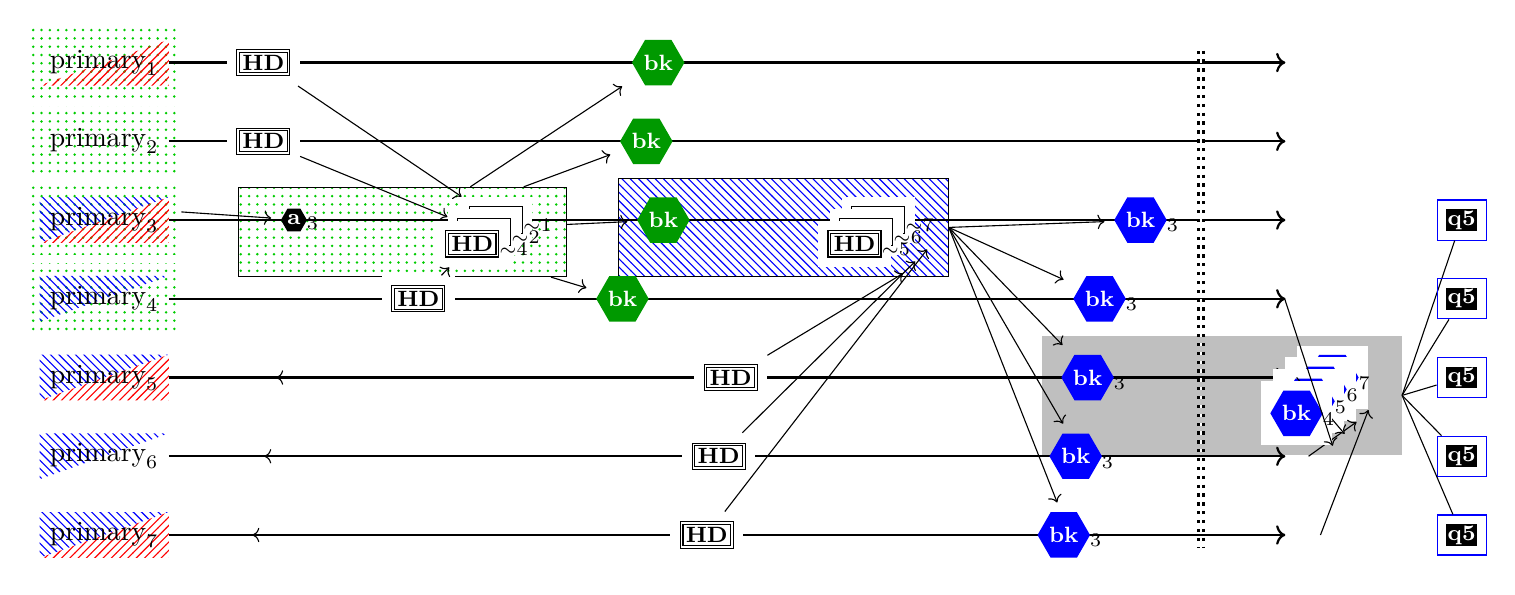
\begin{tikzpicture}[scale=1,thick]
      %%%%%%%%%%%%%%%%%%%%%%%%%%%%%%%%%%%%%%%%%%%%%%%%%%%%%%%%%%%%%%%%%%%%%%%%%%%%%%%% 
      % The message passing diagram of the integrity protocol
      %%%%%%%%%%%%%%%%%%%%%%%%%%%%%%%%%%%%%%%%%%%%%%%%%%%%%%%%%%%%%%%%%%%%%%%%%%% 
      \coordinate (primaryAnchor) at (0,0);
      \foreach \p in {1,...,7} {
        \node[below=\primaryDistance of primaryAnchor,anchor=east] (p\p) 
        at (primaryAnchor) {\ensuremath{\text{primary}_\p}};
        \draw[->] (p\p) -- ++(15,0);
        \coordinate (primaryAnchor) at (p\p.east);
      }
      \begin{pgfonlayer}{background}
        \foreach \p in {1,...,4}{
          \node[pattern=dots, pattern color=green!80!black,fit={(p\p)},inner sep=1ex] {};
        }
        \foreach \p in {1,3,5,7}{
          \fill[pattern=north east lines, pattern color=red]
          (p\p.north east) -- (p\p.south west) -- (p\p.south east) -- cycle;
        }
        \foreach \p in {3,...,7}{
          \fill[pattern=north west lines, pattern color=blue]
          (p\p.north east) -- (p\p.south west) -- (p\p.north west) -- cycle;
        }
      \end{pgfonlayer}

      \node[inner sep = 4ex] (theOrigin) at ([xshift=-3ex]p3.10) {};
      \foreach \p in {1,...,7} { % for each "other" validator
        \coordinate (ac\p') at ([xshift=17ex-\p ex]theOrigin|-p\p) ;
    }
    \node (ac3') at ([xshift=17ex-3 ex]theOrigin|-p3) {\ac\ensuremath{{}_3}};
    \draw[->] (theOrigin) -- ([xshift=4ex,yshift=4ex]ac3'); 
    \coordinate[right=14ex of ac3'] (sigAgg);
    \foreach \p in {1,2,4} { % for each "other" validator
      \node[fill=white] (av\p) at (sigAgg){\hd\makebox[0pt][l]{\ensuremath{{}_{\sim\p}}}};
      \coordinate (sigAgg) at ([xshift=-1ex,yshift=-1ex]sigAgg);
    }
    \foreach \p/\y in {1/2,2/1,4/-14} {
      \node[left=\y ex of ac\p',fill=white] (hd\p') {\hd};
      \draw[->] (hd\p') -- (av\p);
    }
    \begin{pgfonlayer}{background}
      
      \node[fit={(av4)([xshift=2ex]av1.north east)([xshift=-2ex]ac3'.west)},pattern=dots,pattern color=green!80!black,draw] (bkGreen) {};
    \end{pgfonlayer}
    \foreach \p in {1,...,4} { % for each "green" validator
      \node[right=25 ex of ac\p'] (bkGreen\p') {\bk};
      \draw[->] (bkGreen) -- (bkGreen\p'); 
    }
    \foreach \p in {5,...,7} {
      \node[right=35 ex of ac\p',fill=white] (hd\p') {\hd};
      \draw[->] (hd\p') -- (ac\p');
    }
    \coordinate[right=15 ex of bkGreen3'] (sigAgg);
    \foreach \p in {7,...,5} { % for each "other" validator
      \node[fill=white] (av\p) at (sigAgg){\hd\makebox[0pt][l]{\ensuremath{{}_{\sim\p}}}};
      \draw[->] (hd\p') -- ([xshift=1ex,yshift=-.5ex]av\p.south east);
      \coordinate (sigAgg) at ([xshift=-1ex,yshift=-1ex]sigAgg);
    }
      \begin{pgfonlayer}{background}
        
        \node[fit={(bkGreen3')([xshift=2ex]av7.north east)(av5)},pattern=north west lines,pattern color=blue,draw] (bkBlue) {};
      \end{pgfonlayer}
    \foreach \p in {7,...,3} { % for each "blue" validator
      \node[right=65 ex of ac\p'] (bkBlue\p') {\bk[blue]\ensuremath{{}_3}};
      \draw[->] (bkBlue.east) -- (bkBlue\p'); 
    }
    \coordinate (top) at (bkBlue3'.east|-p1); 
    \coordinate (bottom) at (bkBlue3'.east|-p7); 
    \draw[double,very thick,dotted] ([xshift=1ex,yshift=1ex]top) -- ([xshift=1ex,yshift=-1ex]bottom);
    \coordinate (sigAgg) at ([xshift=20ex]bkBlue5');
    \foreach \p in {7,...,4} { % for each "other" blue validator, not 3
      \node[fill=white] (bk\p) at (sigAgg){\bk[blue]\makebox[0pt][l]{\ensuremath{{}_\p}}};
      %\draw[->] (bk\p') -- ([xshift=1ex,yshift=-.5ex]av\p.south east);
      \coordinate (sigAgg) at ([xshift=-1ex,yshift=-1ex]sigAgg);
      \draw[->] (sigAgg|-p\p) -- (bk\p.south east);
    }    
    \begin{pgfonlayer}{background}
      \node[fit={(bkBlue5')([xshift=2ex]bk7.north east)(bk4.south west)},fill=lightgray] (BlueBlocks) {};
    \end{pgfonlayer}
    \foreach \p in {3,...,7} {% for all blue learners
      \node[draw=blue] (qs\p) at ([xshift=5ex]BlueBlocks.east|-p\p) {\qs[5]};
      \draw (BlueBlocks.east) -- (qs\p);
    }
  \end{tikzpicture}%
    \todo{for cooler patternage
      \url{https://tex.stackexchange.com/questions/597172/tikz-set-the-line-width-of-the-pattern}
    }
  }
  \caption[Integrity protocol]{The integrity protocol (fomring the second phase of each round)}%
  % 
  \label{fig:integrity-protocol}
\end{figure}
\todo[inline]{%
  blue blocks go to all validators in 
  %\begin{enumerate}
  % \item
  ① the signing quorum
  % \item
  ② all validators that are in some blue quorum 
  %\end{enumerate}
}

\subsection{Availability: the typical case}

\begin{description}
\item[Generating and broadcasting signed quorums]
  \tnote{primary \\⇒ primary}
  Once a validator has collected 
  enough new  blocks (for a learner), 
  it signs a learner-specific quorum of such blocks;
  the result is called a \emph{signed quorum},  
  for short. 
  All these blocks have to be from the same round. {\color{red} important ‼}

  Under certain conditions,
  in particular if there is exceptional delay for a specific learner,
  one can forgoe announcing a proper signed quorum
  and instead signs a \emph{dummy quorum} for a specific learner,
  \ie a signature over the ID of the learner in question and the current round number.  

\item[General header compilation]
  The biggest additional work and data
  concerns the compilation of headers.
  In the typical phase, 
  a header carries two additional data items, namely
  \begin{itemize}
  \item 
    the availability certificate of the previous header 
    of the header's creator/initiator
  \item 
    hashes of the signed (dummy) quorums sent by the same validator
  \end{itemize}

\item[General header checking]
  As signed quorums also serve as certificates of availability,
  checking a signed quorum amounts to checking the signed certificates.\endnote{%
    Somehow it seems overkill to have (hases of) signed quorums in the headers.   }
  In a similar way,
  the certificate of availability amounts to a checking of signatures.
\end{description}

\todo[inline]{describe in detail how 

  the checking of the availability of the headers takes place}

\subsection{Summary}
The availability protocol in a non-genesis round 
only differs in having
\begin{enumerate}
\item the additional requirement 
that each block header also includes 
the certificate of availability 
for the previous header of the same validator and 
\item 
the sending and checking of signed quorums
(each of which implements the reference to 
blocks from the previous round—in a learner-specific \DAG).
\end{enumerate}

As a consequence,
casting an availability vote / sending a commitment message 
\todo{discuss terminnolgy}
becomes a recursive commitment
to storing all blocks until genesis 
(or the last block that some of learners might still want availabl). 

\section{Data structures}

\begin{figure}[htb]
  \centering
% \subfloat[\color{violet} \bf Missing]{
%   \begin{minipage}{.3\linewidth}
%       \begin{itemize}
%   \item Integrity Vote (cf. Availability Vote → Storing promise ?)
%   \item ~ 
%   \end{itemize}
%   \end{minipage}
% }

  \subfloat[Transaction received by worker~\(w\)]{
    \tx:
    \begin{tikzpicture}[baseline={([yshift=-.5ex]b.center)}]
      \node[ellipse,fill=black] (b){
        \textcolor{white}{\bf\footnotesize\begin{tabular}[c]{c}
                                            trasaction\\
          data
        \end{tabular}}
    };
    \node[anchor=west] (w) at (b.south east) {\small\({}\to w\)};
    \end{tikzpicture}
  }
  \qquad
  \subfloat[Transaction copy (trivial erasure share)]{
    \es: \tx
    % \begin{tikzpicture}[baseline={([yshift=-.5ex]b.center)}]
    %   \phantom{
    %   \node[ellipse,fill=black] (b){
    %     \textcolor{white}{\bf\footnotesize\begin{tabular}[c]{c}
    %       blob\\
    %       of\\
    %       data
    %     \end{tabular}}
    %   };}
    % % https://texample.net/tikz/examples/torn-paper/ 
    % % ‼ make cute torn edges
    % \clip[fill] ([xshift=-1em]b.north east)
    % -- ([yshift=1em]b.south west) 
    % -- ([xshift=1em]b.south west)
    % -- ([yshift=-1em]b.north east) -- cycle;
    % \node[ellipse,fill=black] (b){
    %     \textcolor{white}{\bf\footnotesize\begin{tabular}[c]{c}
    %       blob\\
    %       of\\
    %       data
    %     \end{tabular}}
    %   };
    % \end{tikzpicture}
}
  % \qquad
  % \subfloat[Worker \(y\) is commiting to the hash of~\(x\)]{
  %   \(y♯x\): \([\#(x)]_{\sim y}\)
  % }%‼

\subfloat[Batch hash of worker~\(w\)]{
  \#(\(\overrightarrow\tx\)):
  \#
    \(\left(\begin{tikzpicture}[baseline={(batch.center)}]
      \node[anchor=west] (batch) {
        \(\colorbox{lightgray}{\(\begin{array}[c]{c}
          {\tx}\\%_{\to w}
          {\tx}\\%_{\to w}
          {\tx}\\%_{\to w}
          {\tx}\\%_{\to w}
          {\tx}\\%_{\to w}
          {\tx}%_{\to w}
        \end{array}\)}\)
    };
      \end{tikzpicture}\right)\)
  }
  \subfloat[%
  Worker hash (issued by~\(w\)), 
  including the round number \(\rnd\),
  and the number of transactions~\(\|\protect\overrightarrow \tx\|\);
  it is signed by~\(w\)]{
    \wh:
    \begin{tabular}[t]{@{}l@{}}
      \begin{tikzpicture}[baseline={([yshift=-.5ex]wh.center)}]
        \node (wh){\(\left[ \#(\overrightarrow \tx), \rnd,  \|\overrightarrow \tx\| \right]_{w}\)}; 
      \end{tikzpicture}
      %\footnotesize
    % {\color{violet} + info for correctness checking} \\
    % (\eg number of \tx[s], or list of \#s)\\
    %   \emph{Tahoe – The Least-Authority Filesystem}
    \end{tabular}
  }

  \subfloat[Genesis Header]{
    \(\hd[]\):\(
\tikz[baseline={(x.base)}]{\node (x){
\(\left(p,\overrightarrow\wh\right)\)
};}\)
  }
\qquad
  \subfloat[Genesis certificate of availability]{
    \(\ac\): 
    \(\Bigl[\hd[]\Bigr]_{\overrightarrow q}\)
  }

  \subfloat[Block]{
\bk:
    \begin{math}
      \left[\hd\right]_{\color{green!60!black}{\sim p_1 \dots \sim p_m} [ \color{green!60!black}\sim p_{m+1} \cdots \sim p_{k}]}
    \end{math}
  }
  \qquad
  \subfloat[Signed quorum]{
    \(\qs_p\):
    \begin{math}
      \begin{array}[c]{@{\rhd}l}
        [\bk_1 \cdots \bk_\ell]_{\sim p}
      \end{array}
    \end{math}
  }

  \subfloat[Header]{
    \(\hd\):\(
\tikz[baseline={(x.base)}]{\node (x){
\(\left(p,\overrightarrow\wh,\ac, \overrightarrow {\#(\qsₚ)}\right)\)
};}\)
  }


  \caption{Overview of data structures}
  \label{fig:data-structures}

\end{figure}
\FloatBarrier






\bibliographystyle{alpha}
\bibliography{HN.bib}
\end{document}

\appendix
\printendnotes

\section{food for thought}

\begin{itemize}
\item
  lots of state is completely independent of each other, 
  can we use this for optimization using this ``concurrency''
\item 
  how does this state right tool work ? 
\item 
  How do the message graphs of HP
  compare to Narwhal DAGs
\end{itemize}
\paragraph{Isaac's thoughts}

\begin{itemize}
\item message sharing (on the primary level) might be slow
\item 
\end{itemize}

\href{%
https://github.com/anoma/specs/blob/main/src/architecture/consensus/typhon/mempool.md%
}{the specs}

\section{specific questions}
\begin{itemize}
\item 
  “availability certificate Availability Certificate: an aggregation of signatures from a Weak Quorum attesting that everything referenced by a particular Header is available. \bf Must include a signature from the Header's primary.”
  \begin{itemize}
  \item
\begin{verbatim}
Where is this signature?
\end{verbatim}
  \item
\begin{verbatim}
What does it sign?
\end{verbatim}




  \end{itemize}
\item my acknowledgment, “Availability Vote” --
\begin{verbatim}
isn't it rather a **promise/pledge**
\end{verbatim}
\item about ``blocks'' 
\begin{verbatim}
does it make sense to call these learner blocks, possibly even certified learner blocks?
\end{verbatim}
\item about \tx[s]: 
\begin{verbatim}
  a learner might actually ignore a big chuck of transactions?
\end{verbatim}
\item about the ``two'' protocols
\begin{verbatim}
 if the integrity protocol gets stuck, 
 the availability protocol will stuck?
\end{verbatim}
yes
\begin{verbatim}
   also vice versa ? 
\end{verbatim}
partially 

\item more about blocks
\begin{verbatim}
headers have "sequence numbers" (stemming from the creator)
\end{verbatim}

\item about signed quorum
\begin{verbatim}
would it make sense to call these 
signed_certified learner blocks_
\end{verbatim}
  


\begin{verbatim}
WHEN ARE BLOCKS broadcast and by whom?! 
\end{verbatim}
\color{green!60!black}
it *is* a broadcast and it is performed
\begin{itemize}
\item after completion (in analogy to availability certificates)
\item by the block creator 
\end{itemize}

\end{itemize}

---
\section{Random snippets}

\begin{itemize}
\item Besides the learner graph,
we assume that each transaction is relevant only to a subset of the learners.%
\endnote{%
  \emph{Does it make sense to have transactions that no learner subscribes to?}
  Probaly not! Garbage collection could be triggered by 
}
\ 
\item 
\end{itemize}

---

\begin{description}
\item[New header construction and broadcast] 
  \tnote{primary\\ ⇒ primary}
  The following conditions will trigger the production of a new header.

  \begin{itemize}
  \item
    Each worker on the primary's validator has provided a
    worker has for the validators current round. 
  \item If not genesis round,
    ... %‼ certificate of availability of it's own previous header / block
  \item 
    If not genesis round,
    ...%‼ signed quorum 
  \end{itemize}

  Once, 
  the header is constructed \textcolor{violet}{(but NOT signed?)}, %‼ 
  the primary broadcasts it to all other primaries. 

\item[Header checking and acknowledgment (Availability Vote)]
  A received header of a primary is checked, 
  according to the following check list. 
  
  \begin{itemize}
  \item
    The worker hashes of the header must have been “uploaded”
    by the local workers
    (which are trusted to have check theses worker hashes).
    
  \item If not genesis round,
    ... %‼ certificate of availability of it's own previous header / block
  \item 
    If not genesis round,
    ...%‼ signed quorum 
  \end{itemize}

  After checking all this,
  the primary sents an acknowledment back to the header producer, 
  \ie a message with the header signed. 


\item[Availability Certificate generation and broadcast]
  \tnote{primary\\ ⇒ ∀primary}
  After receiving a global weak quorum of header acknowledments 
  for a previously broadcast header, 
  the received signatures are aggreagated
  \textcolor{violet}{\bf and singed}. %‼ 

  The result is broadcast to all primaries. 

\item[Waiting for (certified learner) blocks]
  \fbox{\color{violet}confusing switch to integrity protocol!}

\item[Announcing signed quorums]
  Once a validator has enough 
  “fresh” blocks (see below) for a learner from a “preceeding” round, 
  the primary signs a learner-specific quorum of such blocks.
  However,
  under certain conditions,
  it might be useful to anounce \emph{empty} signed quorums, 
  indicating that the next block header will not include 
  any signed quorums for a specific learner. 
\end{description}

\subsection{Primary actions in the integrity protocol}
\label{sec:prim-acti-integr}

\begin{enumerate}

\item[Uniqueness attestation / Integrity Vote]
  \tnote{primary\\ → primary}  
  When a primary receives a header from another validator
  with a round number that directly succeeds 
  the last known header of the sending validator, 
  ‼[(for a new \emph{“round”})] %
  the primary signs that header (additionally for the purpose of integerity)
  and sends it back to the creator of the header.

  \color{violet}\item[Certified learner blocks (Integrity certificate for headers)]
  \color{violet}
  \tnote{primary\\ ⇒ primary}
  Upon receiving a learner-specific quorum of integriy votes for a header, 
  the primary aggregates these
  and broadcasts a certied learner block. 

\item[Signed block quorums]
  
  
  


\end{enumerate}


\subsubsection{Genesis round}

\begin{description}
\item[Header compilation]
  \tnote{primary → primary}
  Whenever a full set of worker hashes from another validator
  has ,
  the primary 
  
\end{description}

---

\paragraph{learner-specific round numbers}

\begin{itemize}
\item Each learner might “observe” different round numbers. 
\item In first approximation: do not expect any synchrony whatsoever!
\end{itemize}


\paragraph{reference a quorum of blocks from the previous round}
This is seen as follows,
(for non-genesis blocks):

\begin{itemize}
\item the block contains a header \hd
\item 
\end{itemize}

\paragraph{learner-specific \DAG structure}

\section{Erasure coding}
The worker that has received a transaction from a client
    generates a suitable erasure code,
    broken up into a finite set of shares%
    \footnote{%
      Shares are also known as \emph{chunks}.%
    }%
    \
    to be distributed over all validators. 
    The share distribution has to be such that
    %“
    any quorum of validators (relative to any learner)%
    \endnote{Here, we want to put
    “(relative to any learner \emph{that subscribes to the transaction})”})
    can re-construct the transaction data %
    %”
    from the set of shares 
    that they obtained collectively. %
    %‼ Discuss and give specific example 
    {‼[check this:]\color{red}
    Moreover, 
    the map from 
    erasure coding shares of the transaction
    to (mirror) workers that receive the respective share
    is determined by the worker's index
    (and the identifier of its validator). 
    \todo{\tiny
      %‼ 
      cf. knowing whether we have all the shares ?
    }
    }

\section{State partition and fractal instances}
\label{sec:state-partition}
Learners,
\eg execution engines,
want to be responsible for
\emph{changes} to the smallest possible part of the state.
However,
to enable basic actions such as cross-chain transfers, 
learners have to gather enough information 
about the global state to determine whether 
a given transaction \tx is actually ‼[valid / executable]. 
The matter becomes delicate
if a transaction depends on parts of the state 
that different learners are responsible for. 
No learner can single-handedly determine if
a given commited transaction is executable, 
unless some learner is tracking the complete global state\xspace% 
---an almost impossible task already our days!
Now,
let us focus on transactions whose “inputs” (or “outputs”) are spread out 
over several learners%
\st{ as these are the trouble makers}%
.

\todo[prepend,inline, caption={On chimera chains}]{%
  
★ ``lock'' the relevant parts of the state on all involved learners
\footnote{%
  footnotes in \texttt{\textbackslash todo} notes
  have to be \texttt{\textbackslash protect}ed, 
  unless we put a caption. 
}
 \\
 ★ ``spawn'' a chimera chain\\
 ★ ``move'' locked state fragments to chimera chain\\
 ★ ``settle'' on chimera chain\\
 ★ ``finalize'' chimera chain\\
 ★ ``re-import projected state''
}
% Howevever,
% the validity of a transaction can depend on 
% parts of the state, 
% which lie outside the area of primary interest. 
We assume that each transition carries enough information 
to instantly deduce which part of the global state is accessed,
possibly distinguishing between reading and writing. 


\end{document}

%%% Local Variables:
%%% mode: latex
%%% TeX-master: t
%%% TeX-engine: luatex
%%% TeX-command-extra-options: "-shell-escape"
%%% End:
